\documentclass{article}
\usepackage[utf8]{inputenc}
\usepackage[margin = 0.8in]{geometry}
\usepackage{graphicx}
\usepackage{amsmath, amssymb}
\usepackage{subcaption}
\usepackage{multirow}
\usepackage{mathtools}
\usepackage{float}


\title{RBE550 - Wildfire PRM Assignment}
\author{Keith Chester}
\date{Due date: April 4 2022}

\begin{document}
\maketitle

\section*{Introduction}

In this assignment, we seek to demonstrate path planning with combinatorial and sampling-based methods. Specifically, we utilize A* planning across a continuous space with kinematic constraints of a vehicle across state lattices, and a probabilistic road map method to guide the aforementioned method.

\section*{Vehicles and Kinematics}
We are utilizing an Ackermann steering style vehicle for our robot; specifically modeled after the Mercedes Unimog, a large off roading capable vehicle.

\begin{figure}[H]
    \centering
    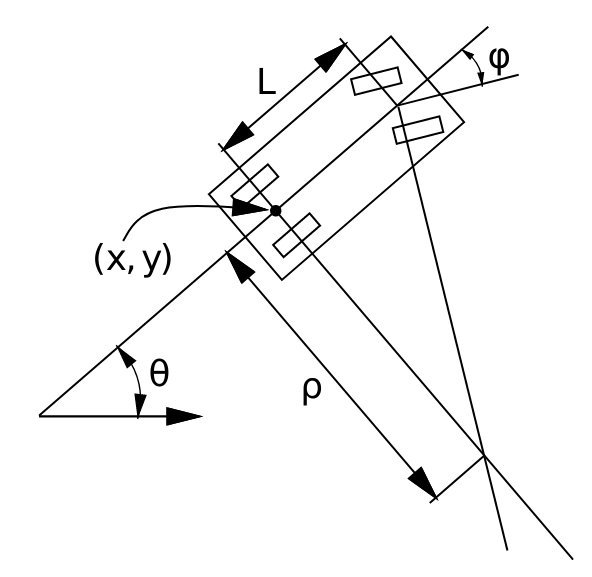
\includegraphics[width = 0.5\textwidth]{imgs/ackermann.png}
    \caption{Ackermann Drive Robot}
    \label{fig:ackermann-drive}
\end{figure}

For our kinematics, we assume that we can control the velocity of our drive wheels in $v$, and the direction of our steering wheels in $\psi$. We limit our steering angles to $\pm 60^o$ and attempt to maintain a speed of $10 \frac{m}{s}$, or $22 mph$. We assume an $L=2.8$ meters.


\begin{equation}
    \dot{\theta} = \frac{v}{L} \tan(\psi)
\end{equation}
\begin{equation}
    \Delta \theta = \dot{\theta} \Delta t
\end{equation}
\begin{equation}
    \theta = \theta_0 + \Delta \theta
\end{equation}
\begin{equation}
    \dot{x} = v \cos(\theta)
\end{equation}
\begin{equation}
    \dot{y} = v \sin(\theta)
\end{equation}
\begin{equation}
    \Delta x = \dot{x} \Delta t
\end{equation}
\begin{equation}
    \Delta y = \dot{y} \Delta t
\end{equation}
\begin{equation}
    x = x_0 + \Delta x
\end{equation}
\begin{equation}
    y = y_0 + \Delta y
\end{equation}

\section*{Simulation and Environment}

Our environment is a self contained $250x250$ meter square area where we have perfect information. Obstacles consist of trees clusterd together into combinations of $15x15$m squares. We assume that an arsonist at $t=0$ and at each $t\%60s=0$ lights fire to a tree at random. Every $20$ seconds, burning trees ignite all trees within $30$ meters. Trees are considered impassable obstacles.

Our simulation can run in real time, or at an accelerated pace where each second of real time results in many seconds in simulation. For the results of this paper, we utilized 1 second of real time is equivalent ot 10 seconds of simulation time, though multiple time equivalences were utilized throughout the development process.

During the planning phase, we paused time in the simulation. We do this as we can not speed up the processor to match simulated processing times, and thus faster simulated time would exaggerate and penalize due to the path planner's calculation time.

\section*{A* Planner Approach}
Here we present a flow chart for the path planner as built. We utilize an A* search algorithm. The act of expanding neighboring cells utilizes kinematic equations for each step to create an in-memory state lattic - this allows us to explore the continuous space as if it was a discrete space.

To store the state lattice and explore its nodes we implemented a priority queue. The cost of each node is the euclidean distance between states from start to this point, and a penalty for $\theta$ changes (to encourage straight movement versus swerving when possible). For a heuristic, we heavily penalize euclidean distance to the goal.

We are not exploring a discrete space, creating a need to identify an acceptable method of determining equality between nodes. To this end we utilized a series of dicts; the $x$ and $y$ location were rounded to the nearest $0.5$ meter, and $\theta$ to the nearest $10^o$. We created an in memory mapping using $defaultdict$, which prevents a $KeyError$ in python, to create a $dict$ ($x$) of a $dict$ ($y$) of a $dict$ ($\theta$) of booleans. This allowed a high speed $O(1)$ lookup if a place was occupied or not.

\begin{figure}[H]
    \centering
    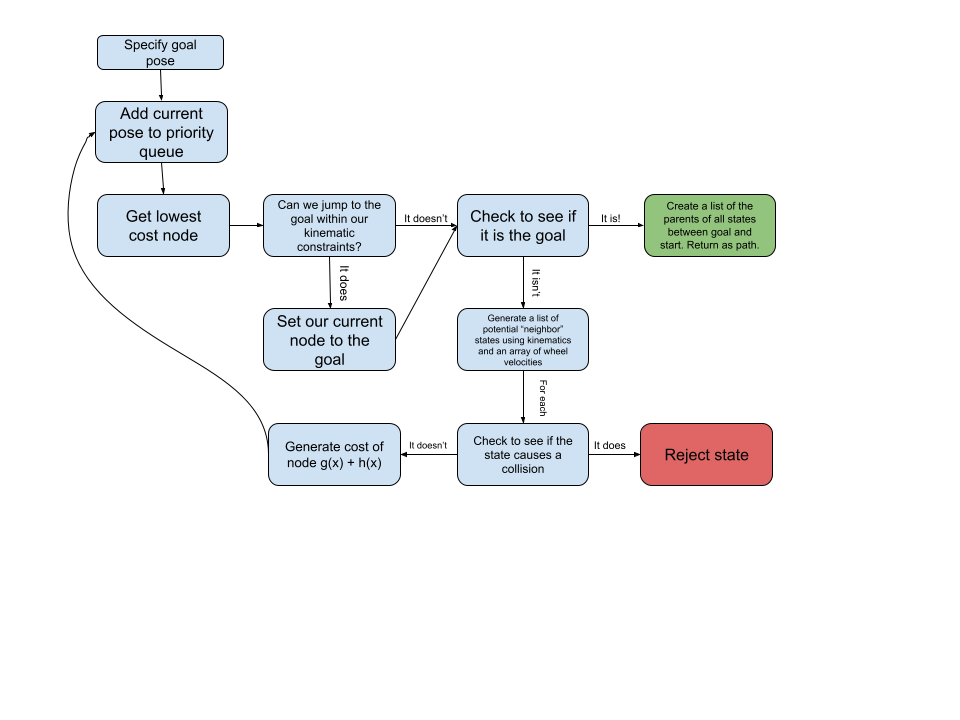
\includegraphics[width = 0.75\textwidth]{imgs/RBE550 Valet flow chart.png}
    \caption{Path planning flow chart}
    \label{fig:path-planning-flowchart}
\end{figure}

\section*{PRM Generation and Planner Approach}

We generated a probabilistic road map (PRM) of our environment to experiment with utilizing it for navigation. We started by generating random $x$ and $y$ points within the $0$ to $250$ meter range. We then chose a random $\theta$ for the vehicle. Finally, we checked if a collision existed in this configuration. If so, we abandon this point and generate another one. If not, we add it to our list of points. We do this for $10,000$ points, as this provided adequate cover we felt.

We stored these points in a $KD-Tree$ - a data structure that provides $O(log(n))$ lookup times for distance querying and nearest point discovery. Since the PRM is static and does not change after initialization, this data structure was ideal for our usage. We utilized the $sklearn$ (Sci-Kit Learn) python module for handling this aspect of the assignment.

From here, we executed A* across the PRM points, with the assumption that each node held a connection with the 5 closest nodes as decided by the $KD-Tree$. Combined with a euclidean distance heuristic for cost, our planner quickly finds the points between nodes within the PRM.

When a burning obstacle is chosen, we find the closest node to it and the vehicle's location. We then utilize the PRM A* planner to find the path amongst the PRM to the objective. We then execute a second A* planner that is identical to our continuous space A* planner described above. Instead of caclulating from the vehicle's location to the goal, we instead task the planner to create a kinematic path moving us between nodes in the PRM.

\section*{Results and Graphs}

In this section we will show the results of our simulation and tests.

In this first set of graphs, we are exploring the total time of calculating a path paired against the euclidean distance from the vehicle to the goal. Note that this may not include pathing through many obstacles despite a short distance, or the amoung of obstacles between the goal and path.


\begin{figure}[H]
    \centering
    \begin{subfigure}{0.4\textwidth}
        \centering
        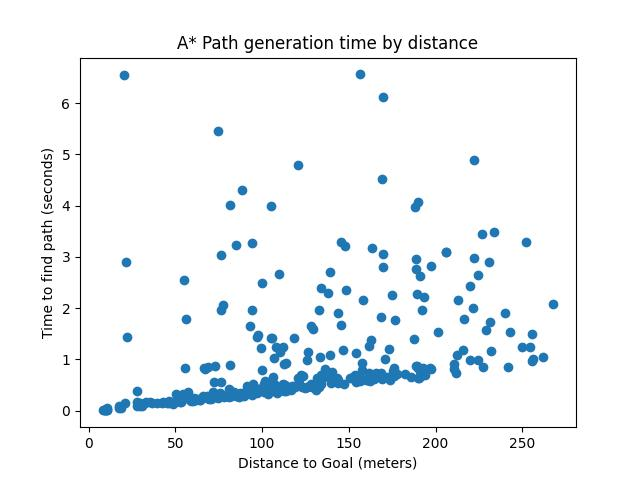
\includegraphics[width = \textwidth]{imgs/astar_paths.jpg}
    \end{subfigure}
    \begin{subfigure}{0.4\textwidth}
        \centering
        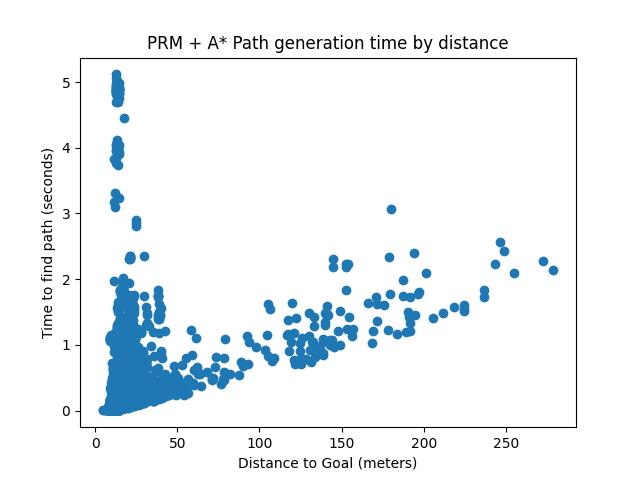
\includegraphics[width = \textwidth]{imgs/prm_paths.jpg}
    \end{subfigure}
    \caption{A* and PRM Path Calculation Time by Distance}
    \label{fig:calc-by-distance}
\end{figure}

On average we saw A* on its own take longer to generate a path, but we saw the PRM method result in several instances of it taking sigificantly longer due to sub-optimal path planning and factors of implementation of the PRM (to be discussed in the Observations section).

In the next set we explore the health of the simulation, and we see that PRM performed worse than A*.

\begin{figure}[H]
    \centering
    \begin{subfigure}{0.4\textwidth}
        \centering
        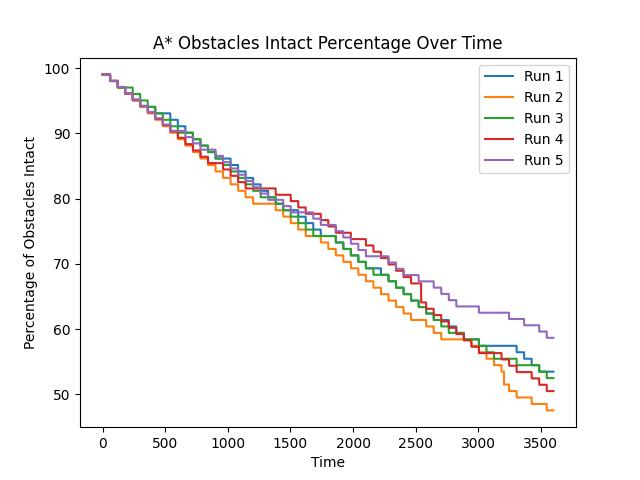
\includegraphics[width = \textwidth]{imgs/astar_obstacles_intact.jpg}
    \end{subfigure}
    \begin{subfigure}{0.4\textwidth}
        \centering
        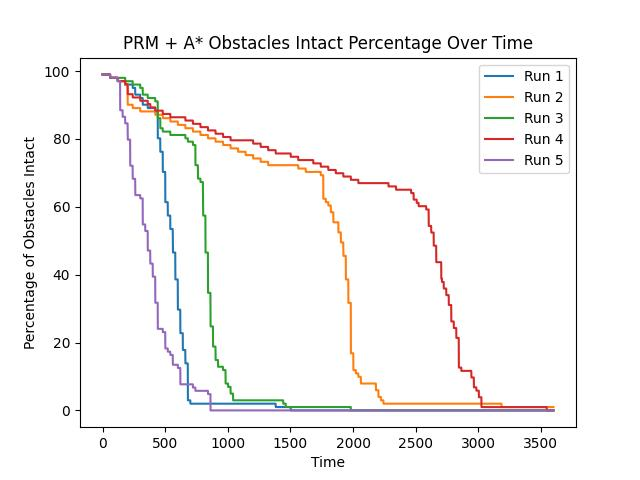
\includegraphics[width = \textwidth]{imgs/prm_obstacles_intact.jpg}
    \end{subfigure}
    \caption{A* and PRM Intact Obstacle Percentage}
    \label{fig:intact}
\end{figure}

An intact obstacle is defined as an obstacle that was never ignited under any circumstance. This graph shows the degradation of the forest over time due to the performance of our machine and the machinations of the arsonist.

\begin{figure}[H]
    \centering
    \begin{subfigure}{0.4\textwidth}
        \centering
        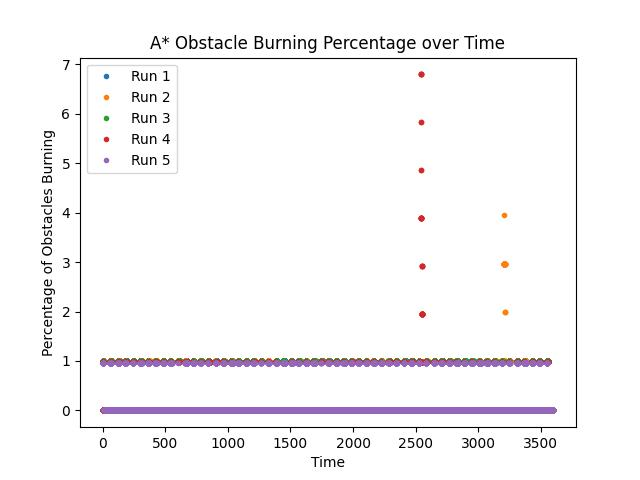
\includegraphics[width = \textwidth]{imgs/astar_obstacles_burning.jpg}
    \end{subfigure}
    \begin{subfigure}{0.4\textwidth}
        \centering
        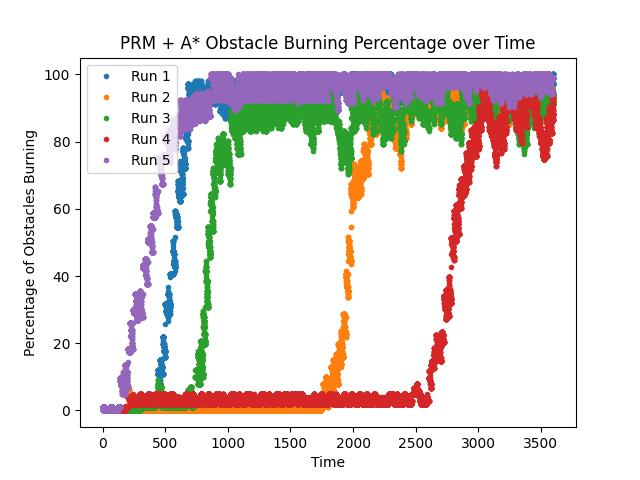
\includegraphics[width = \textwidth]{imgs/prm_obstacles_burning.jpg}
    \end{subfigure}
    \caption{A* and PRM Burning Obstacle Percentage}
    \label{fig:intact}
\end{figure}

Here we see the percentage of obstacles burning at a given moment. Often we see that we go back down to $0\%$, but as the vehicles "lose control" of the environment the fires rapidly spread. A* alone typically outperformed PRM + A*, likely due to reasons discussed below.


\section*{Observations}
We saw improvements and detriments to PRM paired with A* vs A* alone throughout the development and execution of our simulation.

In general, we saw that A* alone performed worse in time to generate a path. Often routing around an obstacle, especially one with nooks, the A* planner would spend too long "focused" on this area before routing around it. The PRM map, having previously established connections instead of trying to map a continuous space, quickly routed around these same obstacles.

PICTURE HERE.

PRM, however, did not result in a consistently better approach for our task at hand. The selection of the node to map to for each obstacle was delegated to the simple algorithm of the closest node to the obstacle's center via the $KD-Tree$. This resulted in a chosen node that may not have been optimal from the current location of the vehicle.

PRM also did not produce optimal paths for to the goal. While it found an optimum path amongst the sampled nodes, this does not gaurantee optimality for the actual space itself. Likewise, the A* planner then must try to find optimal continuous space paths between each node, which may result in sub-optimal paths being generated.

PRM also struggled due to the manner in which we connected nodes within the map. The nodes did not perform adequate collision detection betwen nodes; this meant PRM nodes may be connected that ultimately did not have a viable path between them for the robot to move through. This resulted in occasional tight corridors forcing the A* planner to abandon the PRM's estimated plan and route around the obstacle.

These three reasons resulted in the PRM planner constantly taking longer to reach a goal despite calculating the path to it faster. If we failed to routinely reach an obstacle, we marked it as unreachable. Unfortunately this hampered the PRM planner more, which resulted in more raging fires the vehicle would not put out, which in turn created worse results.

\section*{Conclusion}

In this assignment we looked at the sampling-based method of PRM paired with continuous space planning of A* and state lattices. We tested the algorithms in numerous difficult challenges in random environments.

We saw the benefits and detriments to having a sampling-based map available for path planning, and how choices in implementation can lead to wildly different performance results.

\end{document}